\section{Genetic Programming}
\label{sec:bg:gp}

  \emph{Genetic Programming} (GP)~\autocite{kozaGeneticProgrammingProgramming1992a,kozaGeneticProgrammingII1994,poliFieldGuideGenetic2008a,yuIntroductionEvolutionaryAlgorithms2010}
  has been carved out as a specialized subfield of Evolutionary Algorithms (EAs) 
  which emphasizes evolving a collection of computer programs tailored to address 
  specific problems. While GP can be viewed as a natural evolution of Genetic 
  Algorithms (GAs), it distinguishes itself by its primary goal: GAs streamline 
  parameters to refine a preset function, whereas GP is geared towards program 
  induction.\footnote{%
    A deeper dive into the concept of program induction can be found in \vref{def:program_induction}.
  }

  Beneath the surface, GP and GA exhibit shared principles. Both utilize a population-centric approach, implement a fitness function to gauge the efficacy of individual entities, and harness genetic operators to engender new individuals. However, the way GP represents these individuals, coupled with its distinct genetic operators, sets it apart.

  \begin{remark}
  While GP primarily orbits around a fitness-centric search in the realm of computer programs, its foundational essence is rooted in optimization, echoing the core of GA.
  \end{remark}

  Within the population of GP, every individual is symbolic of a computer 
  program, built from a library of primitives, distinguished as \emph{functions} 
  and \emph{terminals}. To grasp this nuanced structure, picture a composite
  pattern: functions serve as the internal nodes, while terminals act as the leaves (further visual insights can be found in \vref{fig:composite_pattern}). The \emph{abstract syntax tree} (AST) emerges as a fitting representation, where functions are internal nodes and terminals are leaf nodes.

  \begin{figure}[ht!]
    \centering
    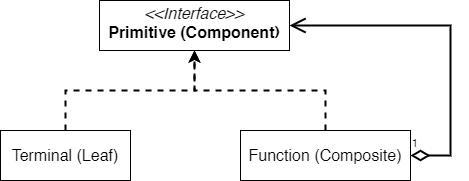
\includegraphics[width=0.4\textwidth]
      {img/theoretical_framework/GP Composite.png}
    \caption{
      A layered visualization of a GP individual, accentuating the interplay
      between functions and terminals.
    }
    \label{fig:composite_pattern}
  \end{figure}

  The GP algorithm, delineated in \vref{lst:bg:gp:algorithm}, bears structural 
  resemblance to the GA algorithm. The key differentiator rests in the specific 
  genetic operations tailored for GP.

  \begin{code}{
    Structural blueprint of the Genetic Programming algorithm, underscoring its 
    architectural alignment with the Genetic Algorithm.
  }{label=lst:bg:gp:algorithm}{kotlin}
    var population = recursively construct random programs
    population.forEach { evaluate and allocate a fitness score }
    while (termination criteria remain unmet) {
      val survivors = cherry-pick survivors(population)
      val parents = select breeding candidates(population)
      val offspring = induce modifications(parents)
      offspring.forEach { evaluate and allocate a fitness score }
      population = merge(survivors, offspring)
    }
    return the cream of the crop from the population
  \end{code}

  In the subsequent segments, we will embark on a meticulous exploration of the 
  pivotal components that breathe life into the GP algorithm, further elucidating 
these concepts with practical illustrations.

\subimport{representation/}{_representation.index.tex}
\subimport{initialization/}{Initialization.tex}
\subimport{selection}{Selection.tex}
\subimport{./variation/}{_variation.index.tex}

\subsection{Deciphering Generalization in GP}
% Elaboration on the concept
% Its significance in the realm of GP
% The pitfalls of overfitting
% Strategies to circumvent overfitting
% Delving into complexity considerations
